\chapter{Introduction}
% Maybe start off as far back as "protein folding"? Perhaps ask Regis about this ... 
% What would I write though?
% Check out Misbehaving proteins the book.

\section{Amyloid}
% The amyloid state of proteins
In vitro, a variety of proteins and peptides, folded or intrinsically disordered, have been found to aggregate to form amyloid fibrils under certain solution conditions. These amyloid fibrils are involved in many incurable human diseases such as prion-related diseases, Parkinson's disease, Huntington's disease, Type II diabetes etc. Furthemore, amyloid have also been known to play beneficial roles in certain living systems. REF

\subsection{Structure}
% In this section I will talk about how amyloid aggregation is thought to work. Introduce the thermodynamic model for understanding fibril formation. I will now broadly introduce amyloid.
% Currently, it is thought that amyloid fibrillar state may be the globally stable folded state for all proteins.

\subsubsection{Fibrils}

\begin{figure}
  \centering
  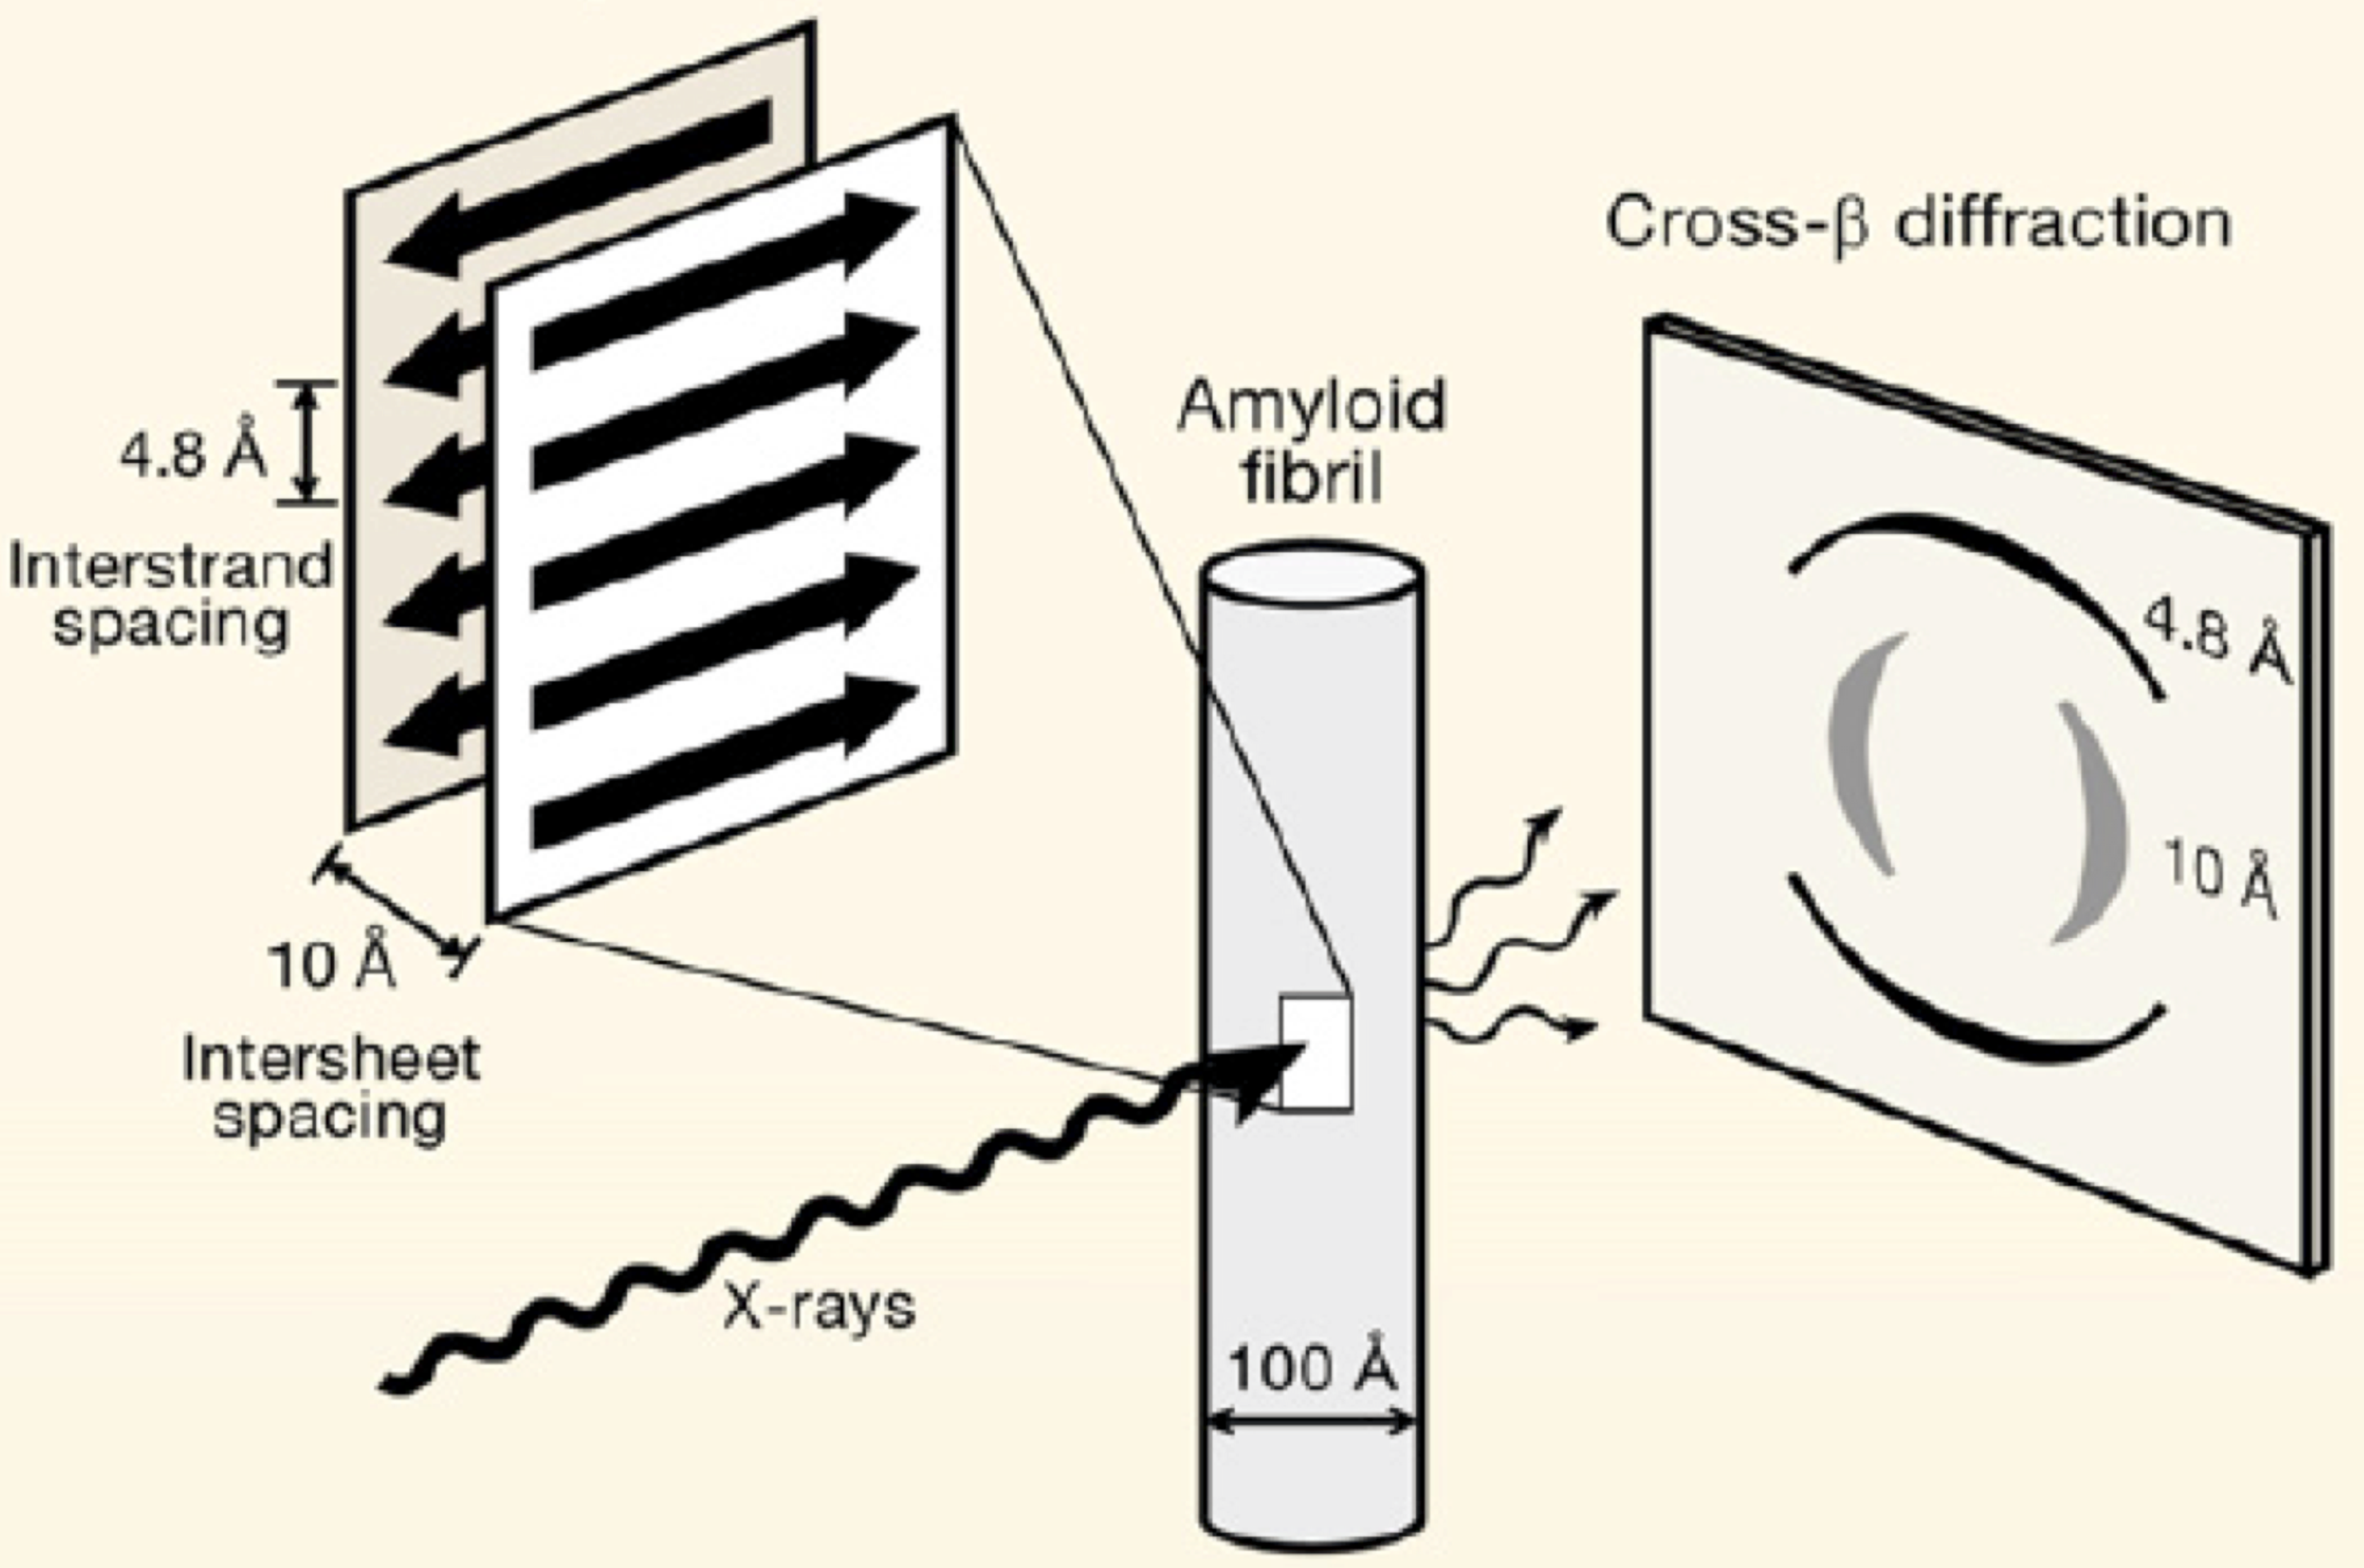
\includegraphics[width=6in]{figures/introduction/fibril_structure_diffraction.pdf}
  \caption[Characteristic cross-$\beta$ spacings from X-ray fibre diffraction studies of amyloid fibrils]{This is adapted from Eisenberg, 2012}
  \label{fig:fibril_diffraction}
\end{figure}

Finding a treatment for AD and other fatal neurodegenerative diseases motivated many biochemical and biophysical studies of the amyloid state. Despite having dramatically differences in sequence, amyloid fibrils formed from different polypeptide all adopt a similar structure. Early structural studies using X-ray diffraction showed that fibrils have a regular structure, with a characteristic 4.8\angstrom\ interpeptide, and 10\angstrom\ intersheet spacing, which have been adopted by biophysicists as the defining characteristic signal for the \crossb\ structure.

Under the transmission Electron microscope (TEM), fibrils are visible as long, ribbon-like structures of about 100 nm in length (Figure~\ref{fig:fibril_TEM_SSNMR}). Independent measurements of fibrillar structure using different instruments have all confirmed the presence of \crossb\ structure as the core structure of amyloid fibrils. (Figure~\ref{fig:fibril_diffraction})

Although \crossb\ is widely known, due to the insolubility and inherent non-crystalline nature of amyloid fibrils, the details of the fibril structure at the molecular level remained elusive until recently. Advances in solid-state NMR and X-ray crystallography in the last decade have made major contributions to our knowledge of the molecular structure of amyloid fibrils.


\begin{figure}
  \centering
  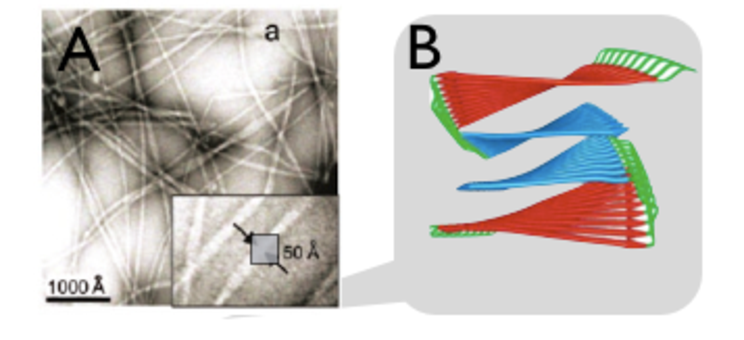
\includegraphics[width=6in]{figures/introduction/fibril_TEM_SSNMR.pdf}
  \caption[Characteristic cross-$\beta$ spacings from X-ray fibre diffraction studies of amyloid fibrils]{A Example EM images of oligomers.  Adapted from Bitan G. et al. 2003 and Walsh D. 1999 C TEM image of fibrils D SSNMR model proposed by Tycko et al.}
  \label{fig:fibril_TEM_SSNMR}
\end{figure}

% Describe the molecular structure of \abeta\ amyloid fibrils. 
% Briefly mention the techniques that can be used to obtain structural information of amyloid fibrils. 

% SSNMR
Both A$\beta$40 and A$\beta$42 amyloid fibrils have been studied in detail using solid-state NMR. Figure~\ref{fig:fibril_TEM_SSNMR}

% X-ray structures
Furthermore, small peptide fragments that have characteristics of amyloid fibrils, which are also amenable to single crystal X-ray diffraction analysis have demonstrated similar type structures from those studied using SSNMR.  These structures obtained by X-ray crystallography have been described to have a dry interface with stacked sheets. (Figure~\ref{fig:fibril_xray_model})

\begin{figure}
  \centering
  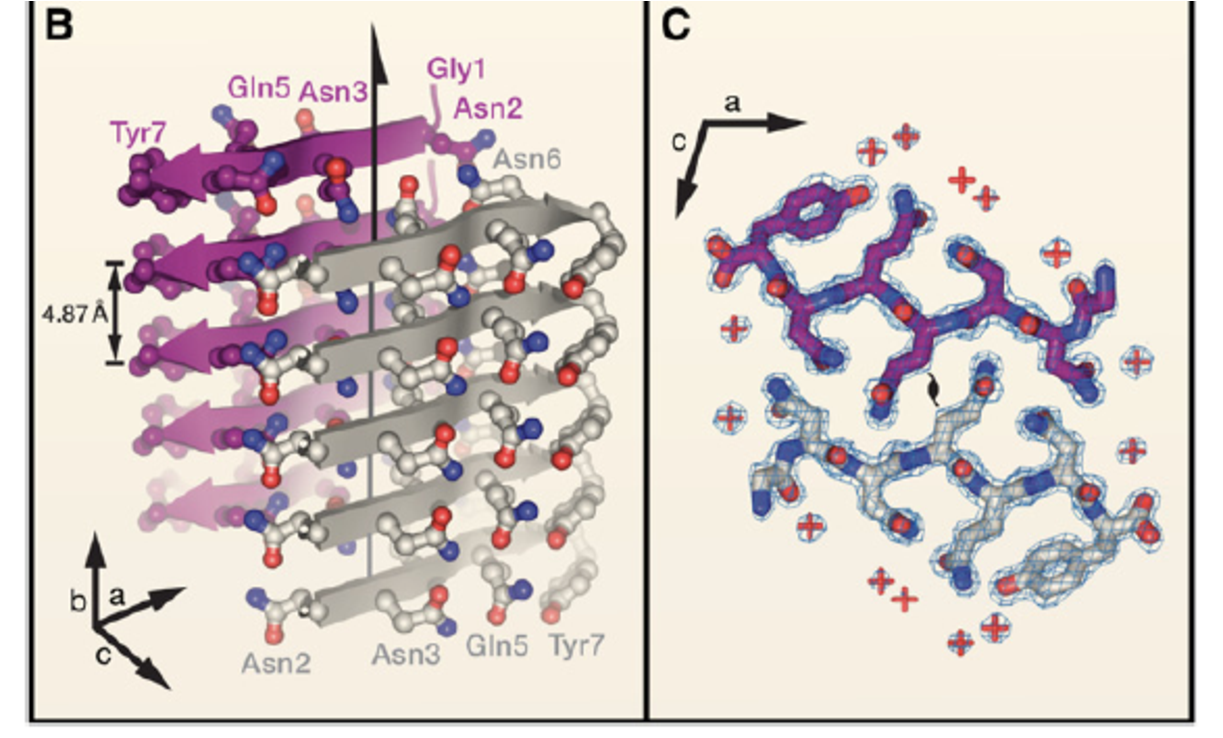
\includegraphics[width=6in]{figures/introduction/fibril_xray_model.pdf}
  \caption[Characteristic cross-$\beta$ spacings from X-ray fibre diffraction studies of amyloid fibrils]{This is adapted from Eisenberg, 2012}
  \label{fig:fibril_xray_model}
\end{figure}


% Fibrils all have the cross beta structure in common
``The ubiq- uitous presence of a cross-β structure strongly supports the view that the physicochemical properties of the polypeptide chain are the major determinants of the fibrillar structure in each case. Moreover, several of the proposed structures, despite very different sequences of their component polypeptides, suggest that the core region is composed of two to four sheets that interact closely with each other. An interesting feature of these sheets is that they appear to be much less twisted than ex- pected from the analysis of the short arrays of β-strands that form β-sheets in globular protein structures. This feature was first pro- posed from cryo-EM and has been supported by Fourier transform infrared (FTIR) analy- ses (48, 61)."

% But fibrils vary in the length of the beta-strand involved, side chain orientation

% Even fibrils formed from a single peptide can exhibit polymorphism due to the different experimental conditions under which they are formed.
Amyloid Fibrils have been found to exhibit polymorphism at the molecular level, but all have similar ultrastructures.  % (Figure~\ref{fig:fibril_diffraction})

		% \1 Decades after the initial discovery by Alois Alzheimer, \abeta, the central protein component of neuronal plaques, was synthetically produced in the laboratory. In vitro, \abeta\ was found to precipitate out of solution almost immediately. 

  \subsubsection{Non-fibrillar oligomers}
   Due to their structural disorder and their insolubility, structural determination of oligomers have posed challenging experimentally.
	
 \subsection{Formation}
% How is amyloid formed
Amyloid fibrils are formed via a complex aggregation pathway. Initially, monomers aggregate to form oligomers with different morphologies which exists in equilibrium with amyloid fibrils. Some of these oligomers are on-pathway to fibril formation, while others themselves may be end-points of the aggregation pathway. Biochemically, fibrils are protease resistant and are insoluble in the presence of SDS.

Amyloid fibrils have been observed to form via a two-step nucleation-polymerization process. In the nucleation phase, energetic barriers of aggregation must be overcome to form the initial aggregation nucleus or seed.  Following nucleation, free monomers bind to the nucleated aggregates and polymerize into mature fibrils.\cite{Murphy:2002fe}

% kinetics of aggregation
\subsection{Involvement in disease}
	% Importance of understanding amyloid.  Role of amyloid in the human body.
Known to be involved in different diseases. Neurodegenerative (AD, Parkinsons, Prion), and diabetes, and systematic amyloidosis.

\subsubsection{Alzheimer's Disease}
% Here, my intention is to lead into the discussion of amyloid by giving a historical perspective and overview of AD
% And use AD as a motivation for why so much work has gone into studying amyloids.

% Clinical symptoms - Cognitive impairment
One of the most well known amyloid disorders is Alzheimer's disease. AD is the most common cause of dementia in persons of age 65 or older. 

With the increasing longevity of our population, AD is approaching epidemic proportions with no cure or preventative therapy available.\cite{Blennow:2006wd}  

MCI progresses to severe memory loss .. what else ...

% Pathological characterization
\begin{figure}
  \centering
  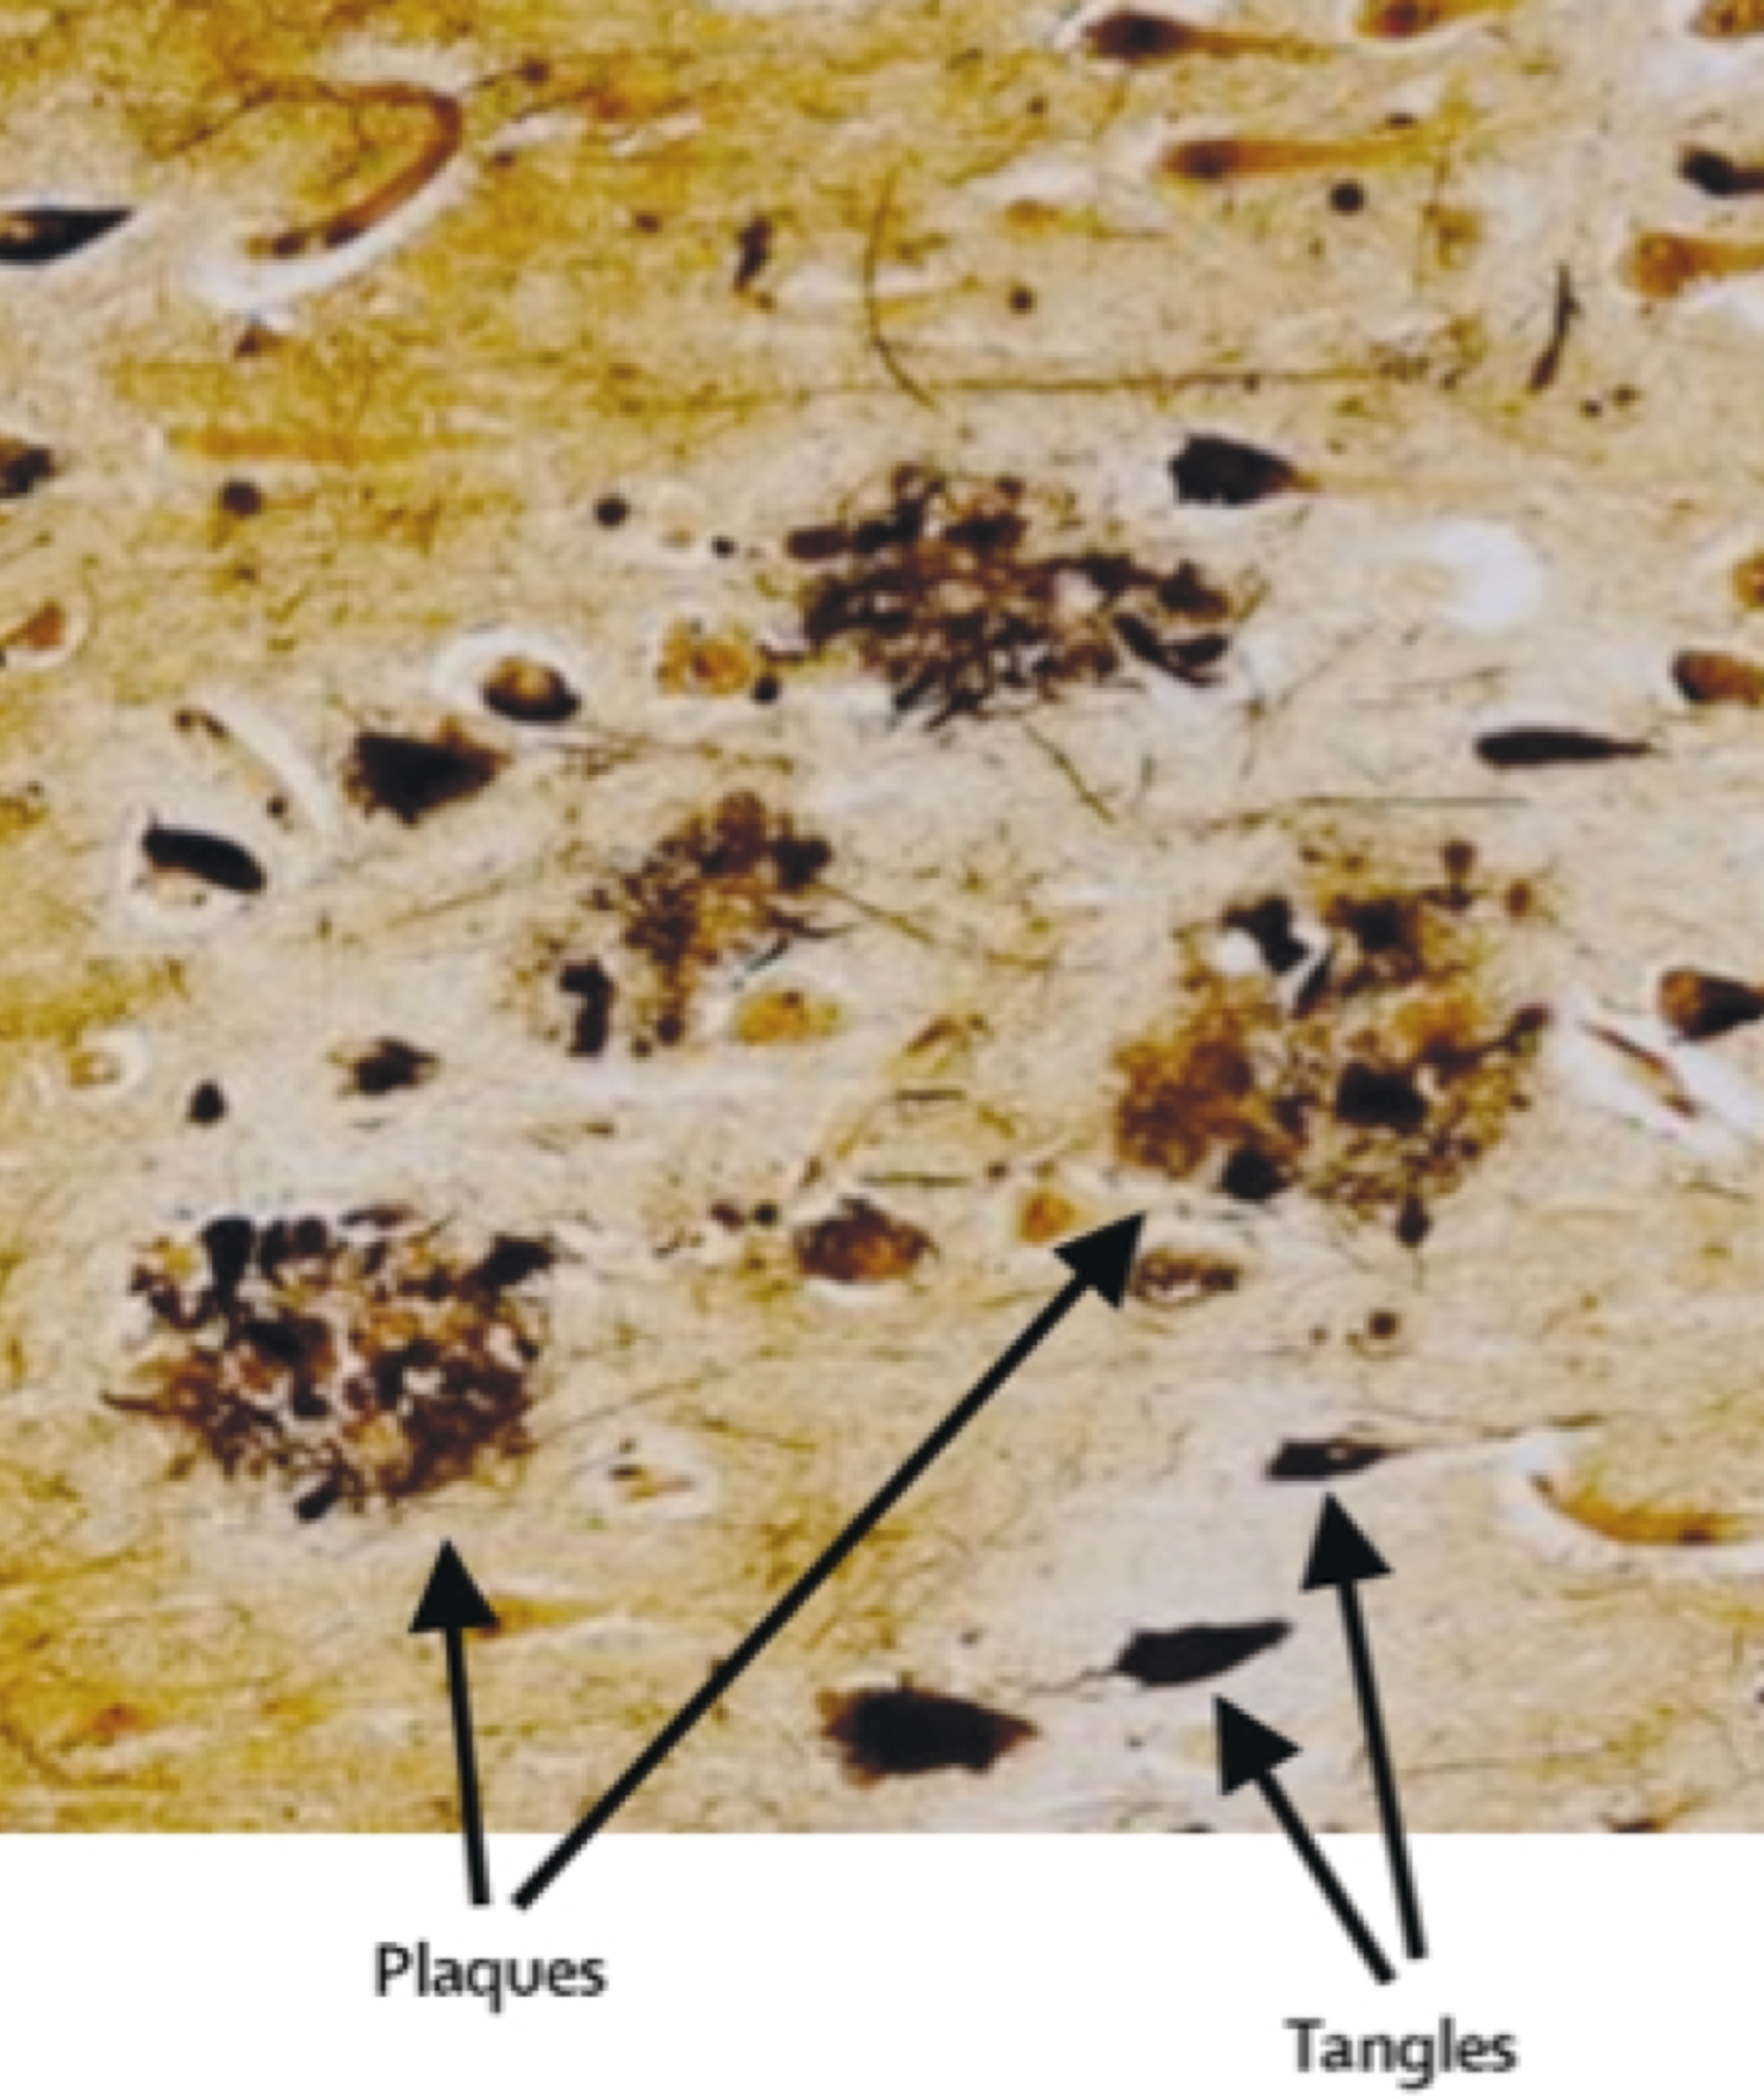
\includegraphics[width=6in]{figures/introduction/AD_tissue_pathology.pdf}
  \caption[Image of lesions formed by plaques and NFTs on brain tissue]{This is adapted from Blennow, 2006}
  \label{fig:AD_tissue_pathology}
\end{figure}

Neuronal dystrophy is often observed upon examination of deceased AD patients. Furthermore, tissue characterization of dementia brains show the presence of extracellular deposits of neuritic senile plaques and neurofibrillary tangles, which appear as lesions on stained brain tissue under light microscopy. (Figure~\ref{fig:AD_tissue_pathology})

Although it has been more than one hundred years since Dr. Alois Alzheimer  first presented the connection between the presence of neuronal plaques and the clinical symptoms of presenile dementia characteristic of Alzheimer's disease (AD), the exact relationship between the two is still under much contention.

% Plaques
It was not until in the 1980s, the protein \abeta\ was identified as the largest component of plaques. \abeta\ aggregates was found to be present in a variety of morphologies in the brain, in fibrillar forms and diffuse forms.

% How is Abeta produced ? Is it only involved in Abeta? What's the physiological role of Abeta?
\abeta\ is produced by intramembrane proteolytic cleavage of the larger amyloid-$\beta$ precursor protein (APP) by $\beta$-secretase, and is produced constitutively as part of the normal cellular metabolism.\{Selkoe, 2002 \#222\} Depending on the position of the cleavage, \abeta peptides of lengths varying from 38 to 43 residues can be produced. However, the peptides spanning residues 1--40 (\abeta40) or 1--42 (\abeta42) are predominantly found AD-associated plaques.

Abeta42 is thought to be more involved in AD than Abeta40.  They oligomerize through different pathways REF. Abeta42 aggregates much faster than Abeta40. 

% BACE

% Plaques and it's Link with amyloid = Abeta
% elaborate on the amyloid hypothesis
The presence of amyloid plaque deposits in brains of deceased dementia patients led to the formulation of the long-standing amyloid hypothesis, which posits that amyloid aggregates initiates the pathogenesis of AD and that the other pathological symptoms such as neurofibrillary tangles are secondary.

% What about NFT's
Although both plaques and NFTs appear, plaques are thought to more likely cause AD than NFT. NFTs involve the aggregation of tau protein.  Several lines of evidence suggest that NFTs plays a secondary role to Abeta in the pathogenesis of AD. Knock out mouse models ... mice do not develop AD, and instead develop tau pathologies NFTs are NFTs have also been shown to be affected by \abeta\ production.

% Diagnosis - hard to diagnose
AD is difficult to diagnose.  It is often not apparent that someone has AD until they exhibit symptoms severe enough to interfere with daily life or occupation. Although plaques are often visible in the dementia patients, plaque load does not appear to correlate well with the progression of disease.  In some individuals without dementia symptoms may have as much plaque as another with severe AD. Synaptic loss can be used as a measure of disease progression. It has been found in recent years that synaptic loss correlates with the concentration of soluble \abeta\ oligomers in the brain.


% Treatment - harder to treat - lack of biochemical understanding of what causes disease, which makes it difficult to develop drugs for; lack of good diagnostic methods because treatment may not be effective at end stages of the disease where brain function won't e able to be rescued.
% Amyloid hypothesis - our best guess at what causes AD and provides the best guess at what we should be targeting. 
% Abeta Amyloid thus far provides the best clue to the molecular basis of AD, and thus a promising pathway to a cure for AD.
Currently there is a lack of treatment which targets the underlying disease. Most approved treatments today for AD are only for mitigating cognitive symptoms. 

Much of the focus on drug development for Alzheimer's has been on preventing amyloid aggregation and decreasing amyloid production.
We will discuss this in more detail in later section XXX.

\subsubsection{Other disorders}
% Perhaps not enough to make it into its own subsection
In addition to AD, other neurodegenerative diseases have been shown to involve the presence of amyloid.  Parkinson's disease, Huntington's, Prion disorders (Mad cow).  These diseases and their pathology are reviewed elsewhere and are beyond the scope of the thesis.


\subsubsection{Toxicity}
% I think outline some of the ideas / hypothesis about the link between amyloid and disease, but don't go into what people speculate or data on toxicity. It is related, but this is out of the scope of your thesis.
\begin{outline}
	% Key question in the field: What is the toxic species?
	\1 Multiple lines of research have identified oligomers as a likely causative agent for neuronal cell death. By contrast, the monomeric and fibril forms are thought to be less toxic than oligomers. It is hypothesized that soluble oligomers may cause toxicity by perturbing the integrity of cellular membranes through binding and disrupting the lipid bilayer (perhaps by making them ion permeable). \cite{Walsh:2007fu}

	\1 Include a paragraph about amyloid formation and lipid membranes (?)
	% Understanding the toxicity or finding out whether there is a toxic species in part validates the amyloid hypothesis. 
\end{outline}


\section{Amyloid Inhibition by small molecules: A promising method of treatment for amyloid disorders}
% Cure, method of prevention; is there hope?

% In this section, I will provide an overview of some of the challenges to overcome when developing a small molecule therapeutic for Alzheimer's disease.  Furthermore, using this information, I will motivate why inositol is an exciting avenue to explore.
	
% Amyloid inhibition as a treatment for Alzheimer's disease and related amyloid disorders. 

% Briefly mention non-small molecule putative therapies which also acts via amyloid inhibition. The focus of this thesis will be on small-molecule amyloid inhibition.

Amyloids are attractive drug targets. Small molecules which targets amyloids may be an effective method of treatment for amyloid disorders because they have the potential to be able to treat the underlying disease. Through in vitro screening, many small molecules have been found to effect the amyloid aggregation pathway.  Some were demonstrated to inhibit amyloid fibrils, where as others were shown to arrest or reduce oligomer formation.
  
% Here I can take a cue from Justin Lemkul`'s recent review paper.
% Talk about the different kinds of small molecules that have been found to inhibition amyloid formation.  Here I will also provide a summary of what people know about the mechanism by which they inhibit amyloid formation.
Pharmacological perspective of the challenge of developing an Alzheimer's drug. In order to effectively treat Alzheimer's and other neurodegenerative diseases, small molecule drug candidates must pass the blood brain barrier at sufficient concentrations for inhibition.  This is difficult to achieve.
      
In vitro screening has led to the discovery of a large number of small-molecules which were found to affect the amyloid aggregation pathway. Many of these small molecules are thought to act by directly binding to amyloidogenic peptides and aggregates.

\begin{figure}
\centering
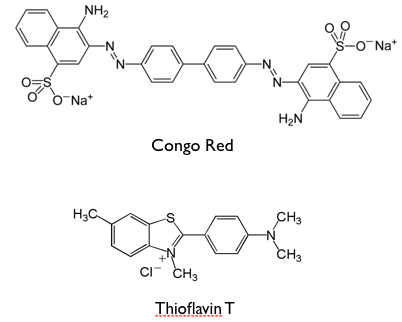
\includegraphics[width=3in]{figures/introduction/dyes.png}
\caption[Small molecule binders]{Amyloid binding dyes Congo Red and Thioflavin T}
\label{fig:amyloid_dyes}
\end{figure}

\subsection{Dye molecules}
Thioflavin T and Congo red are dye molecules used to identify the presence of amyloid.  Both molecules bind to mature amyloid fibrils and have been shown to affect fibril formation.(Fig.~\ref{fig:amyloid_dyes})

\begin{figure}
\centering
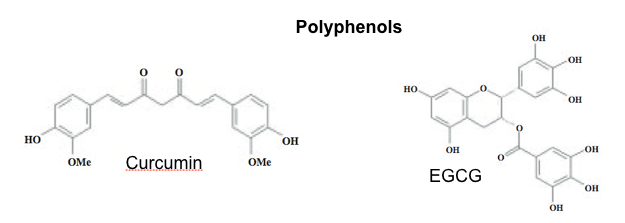
\includegraphics[width=6in]{figures/introduction/polyphenols.png}
\caption[Small molecule binders]{Polyphenols}
\label{fig:polyphenols}
\end{figure}

\subsection{Polyphenols}
Polyphenols,  is a large group of natural and synthetic molecules.  (−)-epigallocatechin-3-gallate, curcumin, and a polyphenolic grape seed extract, known for their anti-oxidant properties,  were recently discovered to be capable of affecting amyloid formation.(Fig.~\ref{fig:polyphenols})

\subsection{Inositol}
\begin{figure}
\centering
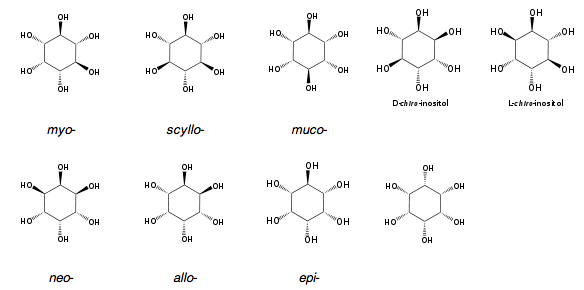
\includegraphics[width=6in]{figures/introduction/inositol.png}
\caption[Inositol]{Inositol stereoisomers}
\label{fig:inositols}
\end{figure}

Inositol stereoisomers.(Fig.~\ref{fig:inositols}) Role of inositol in the human body. \emph{myo}-inositol.  
Inositol is not toxic to the human body.  Inositol is used in signaling pathways. Furthermore, scyllo-Inositol is able to cross the blood brain barrier. It has high bioavailability. Because it is not broken down in the gut, it can be taken orally.

% Use the physiological role of myo-inositol as a lead to transition into its role in amyloid inhibition. 
Inositol stereoisomers are found in various human tissues. It is particularly found at high concentrations in neuronal tissues. Inositol is synthesized inside the body ... or can be obtained via nutrition.  Myo- is present in certain grains, grape fruit, but scyllo- is only found in small quantities in food sources.
	
% Role of inositol in amyloid inhibition. Here, include the background on how inositol was discovered as an \abeta\ amyloid fibril inhibitor.
		
% In vitro and In vivo studies (mouse)
			
% Include some data on human clinical trials (?)

\subsection{Commonalities between small molecule inhibitors}
% Commonalities between small molecules which appear to affect amyloid aggregation
Small molecule inhibitors share common chemical features and groups.  They are typically planar in geometry, have many aromatic rings, and polar functional groups (hydroxyl groups) around the edge of these aromatic rings.



\subsection{Molecular mechanisms of amyloid inhibition 
	            \\ by small molecules}
% Mechanism of action.
Some small molecules inhibit fibril formation, where as others may prevent oligomerization, but not fibrillation. A high concentration is often required to observe activity (micromolar to millimolar), which suggests that they may be non-specific inhibitors. EGCG, one such polyphenol, is known to have the lowest IC50.
    	% IC50 -- This quantitative measure indicates how much of a particular drug or other substance (inhibitor) is needed to inhibit a given biological process (or component of a process, i.e. an enzyme, cell, cell receptor or microorganism) by half.
      % EC50 -- The term half maximal effective concentration (EC50) refers to the concentration of a drug, antibody or toxicant which induces a response halfway between the baseline and maximum after some specified exposure time.[1] It is commonly used as a measure of drug's potency.
      % Ref: wikipedia
      
  	% Review of what is known about amyloid fibril ligand binding, specifically dyes.

Molecular mechanism of binding of dye molecules. Thought to bind flat on on the surface grooves of amyloid fibrils where they interact with hydrophobic groups exposed at the surface. 
      % Doesn't explain why the dye molecules are also able to suppress fibril formation.
      % Can the birefringence be explained by these binding modes? -- this is out of the scope of my thesis.  Don't put this in my thesis but I should be able to coherently explain this during my defense.

\section{Analogy to Sugar-protein binding}
% Does this section fit here? Where should I put it?
% Could use this as a prime example of protein-ligand interaction ...
% As a prime example of protein ligand interaction, one of the first systems that was used to understand binding was a sugar binding protein lysozyme ... -- No I think I will use early systems used to understand protein-ligand binding and if that was a sugar binding protein, then it will come off as a coincidence.
% This section is best discussed in the context of understanding inositol binding ...

% Mention some experimental techniques used to obtain protein sugar-binding modes, but the point here is not to review these methods ... but to point out that I am aware of these techniques.

\subsection{Sugar Binding modes}

% This section provides a nice lead in to the methods section
\section{Protein-ligand interactions}
\subsection{Forces involved in binding}
% Note that I may end up introducing the forces up in the earlier section -- reorganize as needed
\begin{outline}
	\1 Protein-ligand non-covalent interactions that are important for ligand binding and recognition
		\2 Electrostatic interactions. Polar (hydrogen bonding) and charge-charge interactions
		 % Here, it will benefit me to read Sarah's appendix C carefully.
		\2 Nonpolar (hydrophobic) interactions
		  \3 Van der Waals
\end{outline}

\subsection{Binding equilibria}
% subsection protein_ligand_binding_theory (end)
% Below is a summary of an excerpt from Tom's thesis on structure-based drug discovery.
% Design of antibiotics 
% 1) Target determination (biochemical)
% 2) Structural determination (Xray, NMR, or homology); active site identified; Here would be useful to get the holo structure of the protein
% 3) Screen for inhibitors against a chemical library or in silico docking.
\begin{outline}
	\1 Enzyme and its putative ligand typically bind specifically (high affinity binding).  We want to optimize binding specificity to increase the efficacy of the putative drug, and decrease adverse side effects (toxicity) in the human body.

	\1 The dissociation constant, $K_d$, is a measure of the affinity of a ligand for its binding site on the host protein. Pharmacologically, it can be interpreted as the concentration at which 50\% of the drug is bound to the protein. In experimental studies, $K_d$ is often used to quantitatively screen for potential drug candidates. 
  % A small $K_d$ suggests that the ligand may bind tightly to the protein.

	\1 Binding equilibrium

    \begin{equation}
      \left[ Protein\cdot Inositol \right] 
      \rightleftharpoons 
      \left[ Protein \right]+\left[ Inositol \right]
    \end{equation}
  
    % \2 Absolute binding free energy
    % \2 Relative binding free energy
    
	\1 The binding free energy of a ligand to a protein is directly related to its dissociation constant, $K_d$, the equilibrium constant of the above reaction

     \begin{equation}
        K_{d} = f_{ub}\frac{\left[ Protein \right]\left[ Inositol \right]}{\left[Protein \cdot Inositol\right]},
     \end{equation}
     
     % Add equation converting binding constant to gibbs free energies.
	\1 Experimental techniques for estimating $K_d$
		\2 What experimental techniques are used to estimate binding affinity? (May need to study up on this)
		\2 Isothermal titration calorimetry (ITC) is a technique which can be used to measure energetics of ligand binding to peptides.
\end{outline}

% \subsection{Role of chirality in drug binding}
% Stereoisomerism is important to the activity of molecules.  It modulates binding to proteins.
% Two types of stereochemistry
% Constitutional isomers - differs in bonding sequences and connectivity
% Stereoisomers - differs in orientation of their atoms in space, but no connectivity differences.
% Definition of chirality [Add schematic] ... etc
% Molecules with chirality have a non-superimposable mirror image, called an enantiomer.
% A carbon molecule with four different groups has chirality.

\section{Thesis objectives and rationale}
% Understanding amyloid inhibition in the context of the framework of traditional enzyme inhibition mechanism
\subsection{Challenges of amyloid inhibition}
\begin{outline}
       % However, most of these studies were focused on A$\beta$ and large A$\beta$ aggregates,\{Fawzi, 2008 \#553;Esposito, 2008 \#567;Sgourakis, 2007 \#609;Wei, 2006 \#656;Tarus, 2006 \#628 Karsai, 2006 \#658\} and thus, were computationally limited by the complexity of the molecular systems.

    \1 The protein-ligand binding model developed to understand enzyme inhibition cannot be directly applied to understand the molecular mechanism of amyloid inhibition by small molecules. 
    
      \2 Amyloid inhibitors are found to be very weak binders. How do non-specific inhibitors act as a drug? And how do we approach this with MD simulations?
      
      \2  Because the A$\beta$ amyloid aggregate pathway encompasses a variety of species, some of which has no folded structure, a single conformation cannot be assumed for binding. Furthermore, structural information of amyloidogenic species lags behind those of enzymes, which tends to be globular proteins amenable for X-ray crystallography. This means that the putative binding sites are not known.
      
      \2 The structural disorder of the peptides involved poses a challenge for obtaining converged properties from MD simulations. 
    
    	\1 A$\beta$ peptides are completely disordered.  We also do not know what the binding site looks like, where it is located on these structures.
    	
    \1 To date, few studies have attempted to provide statistically meaningful results pertaining to general mechanisms of protein self-aggregation and amyloid formation. Furthermore, despite the abundance of MD studies of A$\beta$, few studies have systematically examined the mechanism of action of small molecule inhibitors of amyloids

    \1 In AD, there is the added challenge of the drug being able to cross the brain barrier, while remaining non-neurotoxic.  What kind of drugs cross the BBB?  Typically hydrophobic drugs.
\end{outline}    

\subsection{Study Design and Rationale}
\begin{outline}
	\1 Here describe in detail how I designed my study to circumvent the challenges presented by the amyloid inhibition problem, and the limitations  of MD simulations. At this point, clearly explain and discuss my study design and rationale. (Fig.~\ref{fig:rationale})

  \begin{figure}
    \centering
    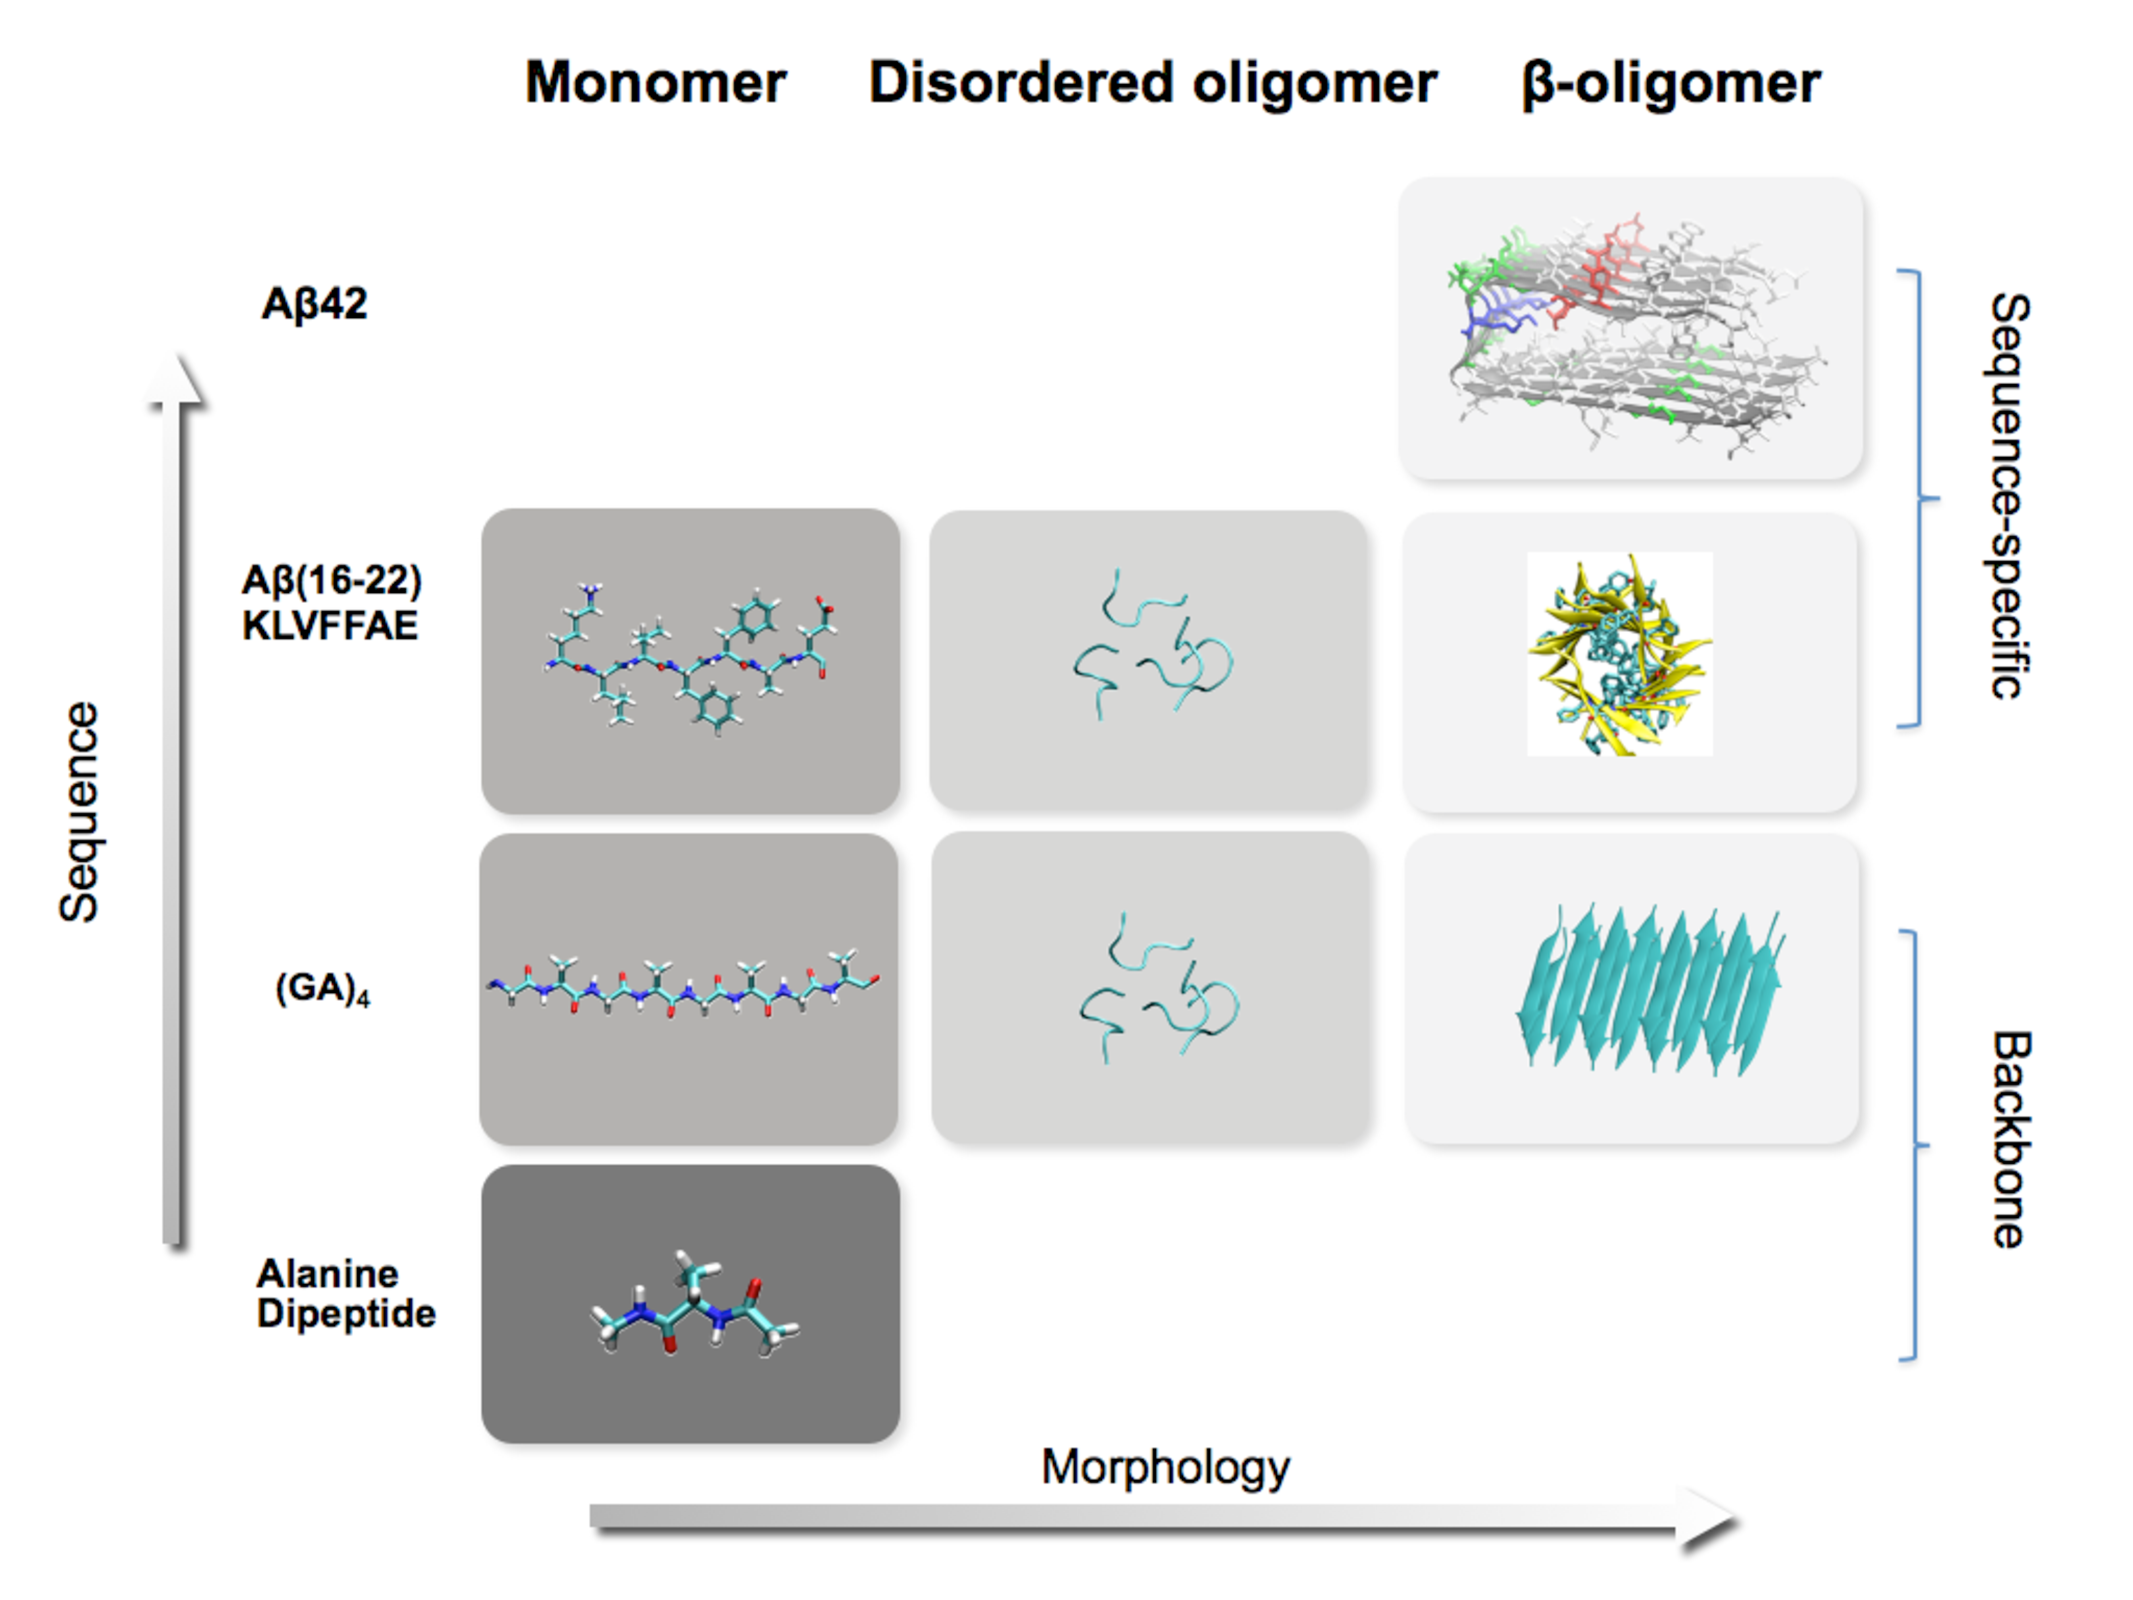
\includegraphics[width=6in]{figures/introduction/matrix.pdf}
    \caption[Rationale]{Shows the progression from small, model systems to larger and structurally more complex systems involving the full-length A$\beta$42 peptide.}
    \label{fig:rationale}
  \end{figure}

	\1 Beginning with the simplest model systems for an amyloidogenic peptide, the alanine dipeptide, we systematically examine binding of inositol with systems of both increasing sequence and structural complexity.

	% Use brute force simulations
	\1 We exploit conventional MD simulation techniques because simulation approaches used for understanding enzyme-ligand binding is not applicable. 
	
	\1 Instead, we use conventional MD simulations and repeats of independent simulations to determine the binding modes, and binding equilibria of inositol with amyloidogenic peptides and aggregates of A$\beta$.
\end{outline}

\section{Thesis Organization}
The first chapter introduces the thesis in the context of the field.  The second chapter introduces the main methods used in the work in the thesis. Chapters 3, 4, and 5 are the results of simulations of inositol with amyloid like peptides and aggregates. Chapter 6 shows work of the general applicability of our methods developed throughout this thesis to MD simulations to understand protein - carbohydrate binding. Chapter 7 provides discussion, suggestions for future work, and perspectives.

\addcontentsline{toc}{section}{Bibliography}
\bibliographystyle{plain}
\bibliography{chapter1}

% \begin{figure}
%   \centering
%   \includegraphics[width=6in]{figures/introduction/fibril_structure_NMR.jpg}
%   \caption[Blah]{NMR model of the core \abeta\ amyloid fibril consistent with MPL from EM, STEM and the cross-$\beta$ structure}
%   \label{fig:fibril_SSNMR_model}
% \end{figure}
